\chapter{Kinematic Equations}

Considering the UAV as a rigid body, the standard kinematic equations can be used. Due to the scope of this analysis, the \textbf{Flat-Earth model} equations will be used, instead of a round Earth (eg WGS-84 model). This option was made since the intended UAV area of operations will be constrained over a small area. GPS coordinates will be used as in a Cartesian grid.

\section{Position}

We express the position vector as
\begin{equation} \label{eq:navshort}
	\bm{p} = [n\ e\ d]^T
\end{equation}
The variables $n$, $e$ and $d$ correspond to the North, East and Down direction, which constitute the primary axis of the NED (as it is called) coordinate system. We shall denote this frame as $\mathcal{F}_F$. The origin of the NED frame is arbitrarily located at the home of operations (or launch point) of every mission and placed on the surface of the Earth.
In contrast, the origin of the so-called body-axes $\mathcal{F}_B$ is the center of gravity point of the aircraft. Its x-axis is placed on the line of longitudinal symmetry, its y-axis starboard and the z-axis downwards, producing a right-handed frame, which can be seen in the following figure.

\begin{figure}[H]
\centering
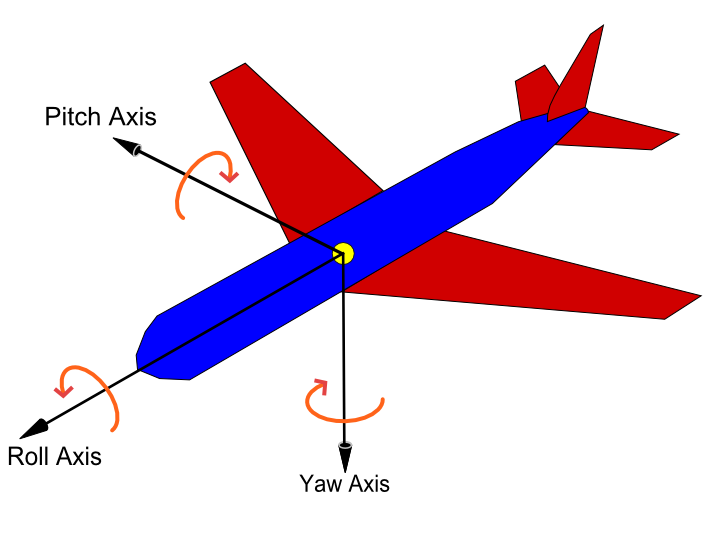
\includegraphics[width=0.45\linewidth]{figures/Plane_Axes}
\caption{Aircraft body axes}
\label{fig:Plane_Axes}
\end{figure}


The derivative of the position is
\begin{IEEEeqnarray}{rCl} \label{eq:posDot}
	\dot{\bm{p}} &= & \bm{R}_b^T \bm{v_i^b}
\end{IEEEeqnarray}
We denote with $R_b$ the transformation matrix \textbf{from the Inertial frame to the Body frame}. Its elements are:

\begin{equation}
\bm{R}_b = \begin{bmatrix}
	\cos \theta \cos \psi                             & \cos\theta \sin\psi                               & -\sin\theta         \\
	-\cos\phi \sin\psi + \sin\phi \sin\theta \cos\psi & \cos\phi \cos\psi + \sin\phi \sin\theta\sin\psi   & \sin\phi \cos\theta \\
	\sin\phi \sin\psi + \cos\phi \sin\theta \cos\psi  & -\sin\phi \cos\psi + \cos\phi \sin\theta \sin\psi & \cos\phi \cos\theta
\end{bmatrix}
\end{equation}


Equation \eqref{eq:posDot} can be broken down onto its three elements as
\begin{IEEEeqnarray}{rCl}
	\dot{n} &= &(\cos \theta \cos \psi) u + (-\cos\phi \sin\psi + \sin\phi \sin\theta \cos\psi) v \nonumber\\
	&& +\> (\sin\phi \sin\psi + \cos\phi \sin\theta \cos\psi)w \IEEEyessubnumber \\
	\dot{e} &= & (\cos\theta \sin\psi)u + (\cos\phi \cos\psi + \sin\phi \sin\theta\sin\psi)v  \nonumber\\
	&& +\> (-\sin\phi \cos\psi + \cos\phi \sin\theta \sin\psi)w \IEEEyessubnumber \\
	\dot{d} &= & (-\sin\theta)u + (\sin\phi \cos\theta)v + (\cos\phi \cos\theta)w \IEEEyessubnumber
\end{IEEEeqnarray}

\begin{lstlisting}[style=C-style]
	dot_north = (cos(theta)*cos(psi))*u + (-cos(phi)*sin(psi)+sin(phi)*sin(theta)*cos(psi))*v + (sin(phi)*sin(psi)+cos(phi)*sin(theta)*cos(psi))*w
	dot_east = (cos(theta)*sin(psi))*u + (cos(phi)*cos(psi)+sin(phi)*sin(theta)*sin(psi))*v + (-sin(phi)*cos(psi)+cos(phi)*sin(theta)*sin(psi))*w
	dot_down = (-sin(theta))*u + (sin(phi)*cos(theta))*v + (cos(phi)*cos(theta))*w
\end{lstlisting}

We see that the rotation matrix $\bm{R_b}$ is dependent upon three variables, $\phi$ , $\theta$ and $\psi$. These are explained below.

In case the linear velocities need to be extracted from the position derivatives, the inverse relation can be used.

\begin{IEEEeqnarray}{rCl}
	u &=& (\cos \theta \cos \psi) \dot{n} + (\cos \theta \sin \psi) \dot{e} + (-\sin \theta)\dot{d} \IEEEyesnumber \IEEEyessubnumber\\
	v &=& (\sin \phi \sin \theta \cos \psi - \cos \phi \sin \psi)\dot{n} \nonumber \\
	&& +\> (\sin \phi \sin \theta \sin \psi + \cos \phi \cos \psi)\dot{e} + (\sin \phi \cos \theta)\dot{d} \IEEEyessubnumber \\
	w &=& (\cos \phi \sin \theta \cos \psi + \sin \phi \sin \psi)\dot{n} \nonumber \\
	&& \> (\cos \phi \sin \theta \sin \psi - \sin \phi \cos \psi)\dot{e} + (\cos \phi \cos \theta)\dot{d} \IEEEyessubnumber
\end{IEEEeqnarray}

\begin{lstlisting}[style=C-style]
	u = (cos(theta)*cos(psi))*dot_n + (cos(theta)*sin(psi))*dot_e + (-sin(theta))*dot_n
	v = (sin(phi)*sin(theta)*cos(psi)-cos(phi)*sin(psi))*dot_n + (sin(phi)*sin(theta)*sin(psi)+cos(phi)*cos(psi))*dot_e + (sin(phi)*cos(theta))*dot_d
	w = (cos(phi)*sin(theta)*cos(psi)+sin(phi)*sin(psi))*dot_n + (cos(phi)*sin(theta)*sin(psi)-sin(phi)*cos(psi))*dot_e + (cos(phi)*cos(theta))*dot_d
\end{lstlisting}

\section{Orientation}

We use Euler angle notation to express the orientation of the aircraft. Roll, pitch and yaw are denoted as $\phi$, $\theta$ and $\psi$ respectively.
\begin{equation}
	\bm{\Phi} = [\phi \ \theta \ \psi]^T
\end{equation}

Figure \ref{fig:Euler_Anlges_2} has a visual representation of those angles. Take a note at the order of rotations: the standard order for aircraft applications, in order to come up with the body frame $\mathcal{F}_B$, starting from the NED frame is:
\begin{enumerate}
\item Rotate around NED z-axis by angle $\psi$, producing frame $\mathcal{F}_1$
\item Rotate around $\mathcal{F}_1$ y-axis by angle $\theta$, producing frame  $\mathcal{F}_2$
\item Rotate around  $\mathcal{F}_2$ x-axis by angle $\phi$, producing the $\mathcal{F}_B$ frame
\end{enumerate}
This convention is called the \emph{Tait-Bryan angles} \cite{Berner2008}

\begin{figure}[H]
\centering
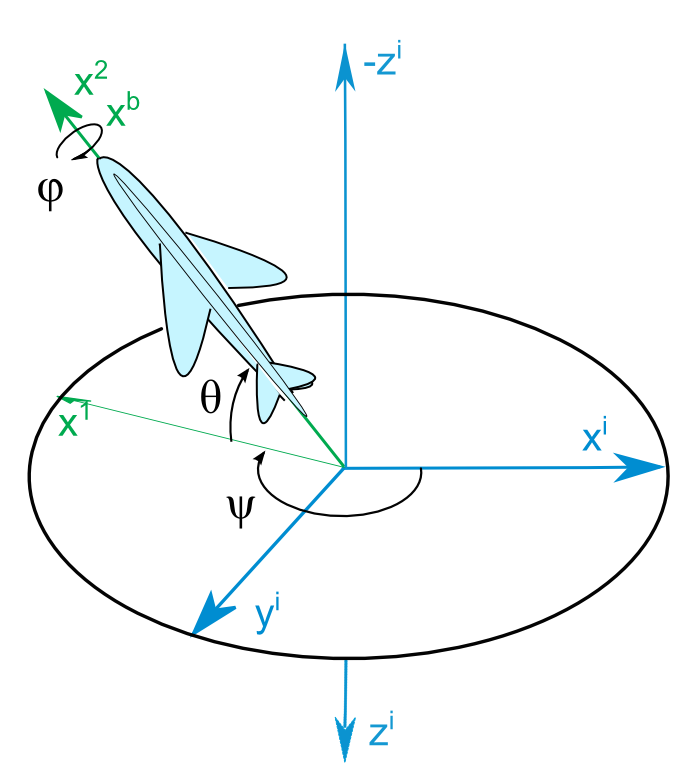
\includegraphics[width=0.35\linewidth]{figures/Euler_Anlges_2}
\caption{Euler angles}
\label{fig:Euler_Anlges_2}
\end{figure}


The time derivative of the Euler angles is
\begin{equation}
	\dot{\bm{\Phi}} = \mathcal{E}(\bm{\Phi})\bm{\omega_b} \label{eq:phi_dot}
\end{equation}
where $\mathcal{E}(\bm{\Phi})$ is a rotation matrix, dependent upon the current orientation.

The individual angle propagation equations are
\begin{IEEEeqnarray}{rCl}
	\dot{\phi} & = & p + \tan\theta \sin\phi q + \tan\theta \cos\phi r \IEEEyessubnumber \\
	\dot{\theta} &= & \cos\phi q - \sin\phi r \IEEEyessubnumber \\
	\dot{\psi} &= & \frac{\sin\phi}{\cos\theta} q + \frac{\cos\phi}{\cos\theta} r \IEEEyessubnumber 
\end{IEEEeqnarray}

\begin{lstlisting}[style=C-style]
	dot_phi = p + (tan(theta)*sin(phi))*q + (tan(theta)*cos(phi))*r
	dot_theta = (cos(phi))*q + (-sin(phi))*r
	dot_psi = (sin(phi)/cos(theta))*q + (cos(phi)/cos(theta))*r
\end{lstlisting}

and equivalenty, $ \mathcal{E}(\bm{\Phi})$ is written as
\begin{equation}
\mathcal{E}(\bm{\Phi}) = \begin{bmatrix}
	1 & \tan \theta \sin \phi        & \tan \theta \cos \phi       \\
	0 & \cos \phi                    & -\sin \phi                  \\
	0 & \frac{\sin\phi}{\cos\theta} & \frac{\cos\phi}{\cos\theta}
\end{bmatrix}
\end{equation}

Inverting \ref{eq:phi_dot} and solving for the angular velocity is possible
%
\begin{IEEEeqnarray}{rCl}
	p &=& \dot{\phi} - \sin \theta \dot{\psi} \\
	q &=& \cos \phi \dot{\theta} + \sin \phi \cos \theta \dot{\psi} \\
	r &=& - \sin \phi \dot{\theta} + \cos \phi \cos \theta \dot{\psi}
\end{IEEEeqnarray}
%
\begin{lstlisting}
	p = dot_phi - sin(theta)*dot_psi
	q = cos(phi)*dot_theta + sin(phi)*cos(theta)*dot_psi
	r = -sin(phi)*dot_theta + cos(phi)*cos(theta)*dot_psi
\end{lstlisting}
\section{Angular velocity}

We define the angular velocity vector as
\begin{equation}
	\bm{\omega} = [p\ q\ r]^T
\end{equation}

and its time derivative is
\begin{equation}  \label{eq:angVelDer}
	\dot{\bm{\omega}} = \frac{1}{\bm{J}}\left(\bm{T_b} - \bm{\omega} \times (\bm{J} \bm{\omega})\right)
\end{equation}

This equation incorporates the inertia matrix $\bm{J}$ and the input torque, expressed in the body axes $\bm{T_b}$.

The inertia matrix is defined as
\begin{equation}
	\bm{J} =
	\begin{bmatrix}
		\int(y^2 + z^2)~dm & -\int xy~dm        & -\int xz~dm        \\
		-\int xy~dm        & \int(x^2 + z^2)~dm & -\int yz~dm        \\
		-\int xz~dm        & -\int yz~dm        & \int(x^2 + y^2)~dm
	\end{bmatrix}
\end{equation}
%
Commonly, the inertia matrix in fixed-wing aircraft is considered to have zero elements in the x-y and y-z direction, since they are symmetric about the x-z plane.
Still, in this section, the full, non-symmetric matrix of inertia will be used, as this is the most general (albeit unlikely) case.
%
\begin{equation}\label{eq:inertiaMat}
	\bm{J} = 
	\begin{bmatrix}
		J_x     & 0   & -J_{xz} \\
		0       & J_y & 0       \\
		-J_{xz} & 0   & J_z
	\end{bmatrix}
\end{equation}

Its inverse is
\begin{equation}
	\bm{J}^{-1} = \frac{1}{det(\bm{J})}
	\begin{bmatrix}
		{j}_{yy}\, {j}_{zz} - {j}_{yz}\, {j}_{zy} & {j}_{xz}\, {j}_{zy} - {j}_{xy}\, {j}_{zz} & {j}_{xy}\, {j}_{yz} - {j}_{xz}\, {j}_{yy}\\
		{j}_{yz}\, {j}_{zx} - {j}_{yx}\, {j}_{zz} & {j}_{xx}\, {j}_{zz} - {j}_{xz}\, {j}_{zx} & {j}_{xz}\, {j}_{yx} - {j}_{xx}\, {j}_{yz}\\
		{j}_{yx}\, {j}_{zy} - {j}_{yy}\, {j}_{zx} & {j}_{xy}\, {j}_{zx} - {j}_{xx}\, {j}_{zy} & {j}_{xx}\, {j}_{yy} - {j}_{xy}\, {j}_{yx}
	\end{bmatrix}
\end{equation}
\begin{lstlisting}[style=C-style]
	Ji[0] = (J[4]*J[8] - J[5]*J[7])/detJ
	Ji[1] = (J[2]*J[7] - J[1]*J[8])/detJ
	Ji[2] = (J[1]*J[5] - J[2]*J[4])/detJ
	Ji[3] = (J[5]*J[6] - J[3]*J[8])/detJ
	Ji[4] = (J[0]*J[8] - J[2]*J[6])/detJ
	Ji[5] = (J[2]*J[3] - J[0]*J[5])/detJ
	Ji[6] = (J[3]*J[7] - J[4]*J[6])/detJ
	Ji[7] = (J[1]*J[6] - J[0]*J[7])/detJ
	Ji[8] = (J[0]*J[4] - J[1]*J[3])/detJ
\end{lstlisting}

where

\begin{equation}
	det(\bm{J}) = \mathrm{j}_{xx}\, \mathrm{j}_{yy}\, \mathrm{j}_{zz} - \mathrm{j}_{xx}\, \mathrm{j}_{yz}\, \mathrm{j}_{zy} - \mathrm{j}_{xy}\, \mathrm{j}_{yx}\, \mathrm{j}_{zz} + \mathrm{j}_{xy}\, \mathrm{j}_{yz}\, \mathrm{j}_{zx} + \mathrm{j}_{xz}\, \mathrm{j}_{yx}\, \mathrm{j}_{zy} - \mathrm{j}_{xz}\, \mathrm{j}_{yy}\, \mathrm{j}_{zx}	
\end{equation}
\begin{lstlisting}{style=C-style}
	detJ = J[0]*J[4]*J8] - J[0]*J[5]*J[7] - J[1]*J[3]*J[8] + J[1]*J[5]*J[6] + J[2]*J[3]*J[7] - J[2]*J[4]*J[6]
\end{lstlisting}

Cross products can be written in matrix form, when implemented as explicit matrix multiplications:
\begin{equation}
\bm{\omega}\times \bm{v} = \begin{bmatrix}
0  & -r & p  \\
r  & 0  & -p \\
-q & p  & 0
\end{bmatrix} \bm{v} =  [\bm{\omega}]_\times \bm{v} \label{eq:matrix_cross}
\end{equation}
%
Where $\bm{v}$ is an arbitrary vector. The notation $[\bm{\omega}]_\times$ represents the skew-symmetric matrix which performs the same matrix operation as the cross product.

Similarly,
\begin{equation}
%
\bm{\omega} \times (\bm{\omega} \times \bm{v}) = \begin{bmatrix}
-r^2-q^2 & pq & pr \\
pq & -p^2 -r^2 & qr\\
pr & qr & -p^2-q^2
\end{bmatrix} \bm{v}
\end{equation}

To facilitate derivations, we define
\begin{IEEEeqnarray}{rCl}
	\bm{C} &=& \bm{\omega}\times(\bm{J}\bm{\omega}) \\
	&=&
		\begin{bmatrix}
			0 & -r & q \\
			r & 0 & -p \\
			-q & p & 0 
		\end{bmatrix} \left(
		\begin{bmatrix}
			j_{xx} & j_{xy} & j_{xz} \\
			j_{yx} & j_{yy} & j_{yz} \\
			j_{zx} & j_{zy} & j_{zz}
		\end{bmatrix}
		\begin{bmatrix}
			p \\ q \\ r
		\end{bmatrix} \right)\\
	&=& \begin{bmatrix}
		q \left(j_{zx} p + j_{zy} q + j_{zz} r\right) - r \left(j_{yx} p + j_{yy} q + j_{yz} r\right)\\ 
		r \left(j_{xx} p + j_{xy} q + j_{xz} r\right) - p \left(j_{zx} p + j_{zy} q + j_{zz} r\right)\\ 
		p \left(j_{yx} p + j_{yy} q + j_{yz} r\right) - q \left(j_{xx} p + j_{xy} q + j_{xz} r\right) 		
	\end{bmatrix}
\end{IEEEeqnarray}

\begin{lstlisting}[style=C-style]
	C[0] = q*(J[6]*p + J[7]*q + J[8]*r) - r*(J[3]*p + J[4]*q + J[5]*r)
	C[1] = r*(J[0]*p + J[1]*q + J[2]*r) - p*(J[6]*p + J[7]*q + J[8]*r)
	C[2] = p*(J[3]*p + J[4]*q + J[5]*r) - q*(J[0]*p + J[1]*q + J[2]*r)
\end{lstlisting}


and
\begin{equation}
	\bm{J}^{-1} =
	\begin{bmatrix}
		j^i_{11} & j^i_{12} & j^i_{13} \\
		j^i_{21} & j^i_{22} & j^i_{23} \\
		j^i_{31} & j^i_{32} & j^i_{33}
	\end{bmatrix}
\end{equation}

Thus, \ref{eq:angVelDer} becomes
\begin{IEEEeqnarray}{rCl}
	\dot{\bm{\omega}} &=&
	\begin{bmatrix}		
		j^i_{11} & j^i_{12} & j^i_{13} \\
		j^i_{21} & j^i_{22} & j^i_{23} \\
		j^i_{31} & j^i_{32} & j^i_{33}
	\end{bmatrix}
	\left(
	\begin{bmatrix}
		T_x \\ T_y \\ T_z
	\end{bmatrix} - 
	\begin{bmatrix}
		c_{1} \\
		c_{2} \\
		c_{3}
	\end{bmatrix}
	\right) \Leftrightarrow \\
	&=&  \begin{bmatrix}
		j^i_{11} \left(T_x - c_{1}\right) + j^i_{12} \left(T_y- c_{2}\right) + j^i_{13} \left(T_z - c_{3}\right)\\
		j^i_{21} \left(T_x - c_{1}\right) + j^i_{22} \left(T_y - c_{2}\right) + j^i_{23} \left(T_z - c_{3}\right)\\
		j^i_{31} \left(T_x - c_{1}\right) + j^i_{32} \left(T_y - c_{2}\right) + j^i_{33} \left(T_z - c_{3}\right)
	\end{bmatrix}	
\end{IEEEeqnarray}

\begin{lstlisting}[style=C-style]
	dot_p = Ji[0]*(T_x-C[0]) + Ji[1]*(T_y - C[1]) + Ji[2]*(T_z - C[2])
	dot_q = Ji[3]*(T_x-C[0]) + Ji[4]*(T_y - C[1]) + Ji[5]*(T_z - C[2])
	dot_r = Ji[6]*(T_x-C[0]) + Ji[7]*(T_y - C[1]) + Ji[8]*(T_z - C[2])
\end{lstlisting}

Conversely, if needed, we can write
\begin{IEEEeqnarray}{rCl}
	\bm{T}_b &=& \bm{J}\dot{\bm{\omega}} + \bm{\omega}\times\left( \bm{J}\bm{\omega} \right) \Leftrightarrow \\
	\bm{T}_b &=& \bm{J}\dot{\bm{\omega}} + \bm{C} \Leftrightarrow \\
	\begin{bmatrix}
		T_x \\ T_y \\ Tz
	\end{bmatrix}
	& = &
	\begin{bmatrix}
		j_{xx} & j_{xy} & j_{xz} \\
		j_{yx} & j_{yy} & j_{yz} \\
		j_{zx} & j_{zy} & j_{zz}
	\end{bmatrix}
	\begin{bmatrix}
		\dot{p} \\ \dot{q} \\ \dot{r}
	\end{bmatrix}
	+
	\begin{bmatrix}
		c_{1} \\
		c_{2} \\
		c_{3}
	\end{bmatrix}
\end{IEEEeqnarray}
%
and in scalar form
%
\begin{IEEEeqnarray}{rCl}
	T_x &=& j_{xx}\dot{p} + j_{xy}\dot{q} + j_{xz}\dot{r} + c_1 \\
	T_y &=& j_{yx}\dot{p} + j_{yy}\dot{q} + j_{yz}\dot{r} + c_2 \\
	T_z &=& j_{zx}\dot{p} + j_{zy}\dot{q} + j_{zz}\dot{r} + c_3
\end{IEEEeqnarray}
%
\begin{lstlisting}
	T_x = J[0]*dot_p + J[1]*dot_q + J[2]*dot_r + C[0]
	T_y = J[3]*dot_p + J[4]*dot_q + J[5]*dot_r + C[1]
	T_z = J[6]*dot_p + J[7]*dot_q + J[8]*dot_r + C[2]
\end{lstlisting}


\section{Linear Velocity}

We define inertial linear velocity expressed in the body frame and its components as
\begin{equation}
	\bm{v}_i^b = [u\ v\ w]^T
\end{equation}
The inertial linear velocity expressed in the inertial frame is, as we saw earlier
\begin{equation}
	\bm{v}_i^i = [\dot{n}\ \dot{e}\ \dot{d}]^T
\end{equation}
The norm of the inertial linear velocity is
\begin{equation}
	V_i = \lVert [u\ v\ w] \rVert = \lVert [\dot{n}\ \dot{e}\ \dot{d}] \rVert
\end{equation}
%
\begin{lstlisting}
	V_i = sqrt(u*u + v*v + w*w)
	V_i = sqrt(dot_north*dot_north + dot_east*dot_east + dot_down*dot_down)
\end{lstlisting}

Sometimes, the projection of the inertial velocity on the North-East plane is of interest and two more quantities accompany it. First, we define the \textit{course angle} $\chi$, as the angle that the projection of the UAV trajectory on the North-East plane has at any time in terms of the North direction. The \textit{flight path angle} $\gamma$ is the angle between the inertial velocity vector and the North-East plane. Finally, the \textit{ground velocity} is defined as the norm of the projection of the inertial velocity vector on the North-East plane.
%
\begin{IEEEeqnarray}{rCl}
\chi &=& \operatorname{atan2}\left({\dot{e}},{\dot{n}}\right) \\
\gamma &=& \operatorname{asin}\left({-\dot{d}}/V_i\right) \label{eq:gamma}\\
V_g &=& V_i \cos \gamma
\end{IEEEeqnarray}
%
\begin{lstlisting}
	chi = atan2(dot_east, dot_north)
	gamma = asin(-dot_down/V_i)
	V_g = V_i*cos(gamma)
\end{lstlisting}
%
The negative sign in \ref{eq:gamma} maintains the convention where increase in altitude should correspond to positive $\gamma$ values, while at the same time $\dot{d}$ decreases.

The time derivative of the inertial velocity expressed in the body frame is
\begin{equation}
	\dot{\bm{v}_i^b} = -\bm{\omega^b} \times \bm{v}_i^b + \frac{\bm{F_b}}{m}
\end{equation}

which is equivalent to
\begin{IEEEeqnarray}{rCl}
	\dot{u} &= & rv -qw + \frac{F_{b,x}}{m} \IEEEyessubnumber \\
	\dot{v} &= & -ru + pw + \frac{F_{b,y}}{m} \IEEEyessubnumber \\
	\dot{w} &= & qu -pv + \frac{F_{b,z}}{m} \IEEEyessubnumber
\end{IEEEeqnarray}

\begin{lstlisting}[style=C-style]
	dot_u = r*v - q*w + F_x/m
	dot_v = -r*u + p*w + F_y/m
	dot_w = q*u - p*v + F_z/m
\end{lstlisting}

We need to define the wind velocity, in the body frame. This is the velocity of the air-mass, moving above the ground, expressed in the body axes.
\begin{equation}
	\bm{v}^w = [u_w\ v_w\ w_w]^T
\end{equation}

The resulting relative (air)speed of the aircraft is
\begin{equation}
	\bm{v}_r = \bm{v}_i^b - \bm{v}_w
\end{equation}

\begin{lstlisting}[style=C-style]
	u_r = u - u_w
	v_r = v - v_w
	w_r = w - w_w
\end{lstlisting}

Relative velocity is a very important quantity in aeronautics, as every aspect of the aircraft's aerodynamic response depends on it, rather than the inertial speed.

Based on the relative velocity, we define three more quantities:
\begin{itemize}
\item the angle of attack, $\alpha$
\item the angle of sideslip, $\beta$
\item the airspeed, $V_a$
\end{itemize}


\begin{IEEEeqnarray}{rCl}
	\alpha &= &\tan^{-1} \left(\frac{w_r}{u_r}\right) \IEEEyesnumber \IEEEyessubnumber \\
	\beta &= &\sin^{-1}\left(\frac{v_r}{V_a}\right) \IEEEyessubnumber \\
	V_a &= &\lVert[u_r\ v_r\ w_r]^T\rVert
\end{IEEEeqnarray}

\begin{lstlisting}[style=C-style]
		alpha = atan2(w_r,u_r)
		beta = asin(v_r/V_a)
		V_a = sqrt(u_r*u_r + v_r*v_r + w_r*w_r)
\end{lstlisting}

\todo[inline]{Cross-reference with \cite[p~208]{Laban1994}}

Using these angles, a new frame of reference can be constructed, the Stability frame $\mathcal{F}_S$. The relative speed components (expressed in the body frame) can be constructed from the airspeed (expressed in the stability frame) using the following rotation:

\begin{equation}
\bm{v}_r = \bm{S}^T \begin{bmatrix}
V_a \\ 0 \\ 0
\end{bmatrix}
\end{equation}

\begin{equation}\label{eq:StabMatrix}
	\bm{S}=
	\begin{bmatrix}
		\cos\alpha \cos\beta & \sin\beta & \sin\alpha \cos\beta \\
		-\cos\alpha \sin\beta & \cos\beta & -\sin\alpha \sin\beta \\
		-\sin\alpha & 0 & \cos\alpha
	\end{bmatrix}
\end{equation}



\section{Mass Distribution}

It is useful to model the mass distribution of our aircraft. It has a nominal mass $m_{nom}$, placed at the center of mass, the origin of the body axes. Any extra weights, such as payloads, debris, or component detachment can be modeled with extra masses $m_i$. Under this definition, $m_i$ is allowed to be negative.
The overall mass and center of mass location are:

\begin{IEEEeqnarray}{rCl}\label{eq:masses}
	m &= & m_{nom} + \sum m_i \IEEEyesnumber \IEEEyessubnumber \\
	\bm{p}_{m,{nom}} &= &[0\ 0\ 0]^T \IEEEyessubnumber \\
	\bm{p}_{CM} &= & \frac{1}{m} \left( \sum \bm{p}_{m_i} m_i\right)
\end{IEEEeqnarray}

\begin{lstlisting}[style=C-style]
	m = m_nom + m_i
	p_cm_x = 1/m*(p_mi_x*m_i)
	p_cm_y = 1/m*(p_mi_y*m_i)
	p_cm_z = 1/m*(p_mi_z*m_i)
\end{lstlisting}

The shifts in center of mass affect the dynamic response of the aircraft and should be taken into account. Consider Figure \ref{fig:CG_shift} where in the nominal case on the left, a thrust force is applied on the propeller. The force is aligned with the center of mass, thus no torque is generated. Now let's consider an edge case, where a very dense, heavy point mass has been added to the tip of the right wing. The center of mass of the airplane is now about midway of the right wing. As a result, the thrust force will now apply a torque on the z-axis, which needs to be covered by our modeling.

One approach which would not bring the required results would be to leave the nominal CoM in its original place and model the extra mass as a separate body, which is subject to gravity force. This force would be added to the force balance and, due to its lever on the CoM, it would also apply torque, weighing the right wing down. However, the torque produced by the thrust force cannot be created with this modeling.

The correct approach is to re-calculate the location of the center of mass, as per \ref{eq:masses}. Gravity is still considered to not exert any moments on the aircraft body, but now there is a level on the thrust force, which will correctly produce torque. The same holds with the lift force, which is applied on the center of lift and will produce a rolling moment to the right.

\begin{figure}\label{fig:CM_shift}
\centering
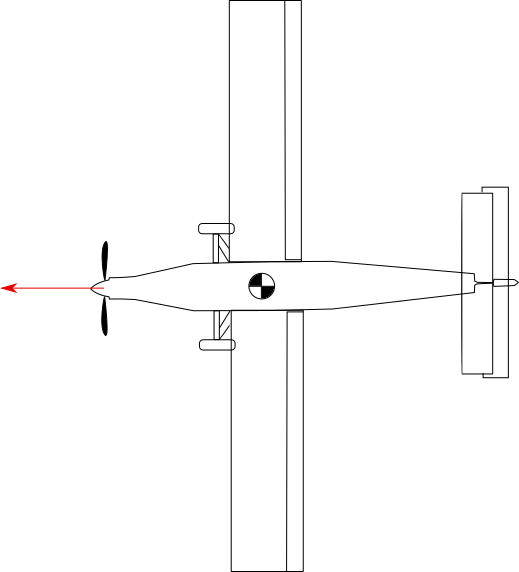
\includegraphics[width=0.4\linewidth]{figures/CG_shift_normal}
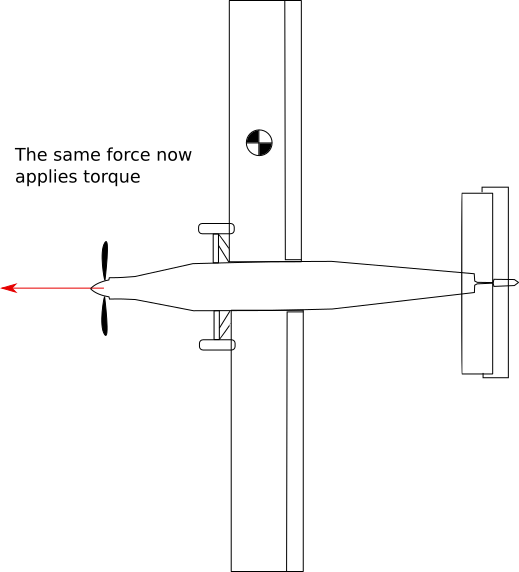
\includegraphics[width=0.4\linewidth]{figures/CG_shift_shifted}
\caption[The effect of CoM shift]{The effect of CoM shift}
\label{fig:CG_shift}
\end{figure}

Naturally, mass additions also affect the matrix of inertia of the aircraft. A mass $m_{i}$ planted at the point $p_{m_i} = [x_{m_i}, y_{m_i}, z_{m_i}]^T$ perturbs the matrix of inertia additively by \cite{wiki:inertia_matrix}
%
\begin{equation}
	\Delta \bm{J}_{mi} = - m_i [p_{m_i}]_\times^2
\end{equation}
%
which, according to \ref{eq:matrix_cross}, in matrix form is
%
\begin{equation}
	\Delta \bm{J}_{m_i} =
	\begin{bmatrix}
		(y_{m_i}^2 + z_{m_i}^2) m_{i} & -x_{m_i} y_{m_i} m_i         & -x_{m_i}z_{m_i}m_i          \\
		-x_{m_i} y_{m_i} m_i          & (x_{m_i}^2 +  z_{m_i}^2) m_i & -y_{m_i} z_{m_i} m_i        \\
		-x_{m_i}z_{m_i}m_i            & -y_{m_i} z_{m_i} m_i         & (x_{m_i}^2 + y_{m_i}^2) m_i
	\end{bmatrix}
\end{equation}

%\begin{lstlisting}[style=C-style]
%	J_delta_i[0] = (y_mi*y_mi+z_mi*z_mi)*m_i
%	J_delta_i[1] = -x_mi*y_mi*m_i
%	J_delta_i[2] = -x_mi*z_mi*m_i
%	J_delta_i[3] = -x_mi*y_mi*m_i
%	J_delta_i[4] = (x_mi*x_mi+z_mi*z_mi)*m_i
%	J_delta_i[5] = -y_mi*z_mi*m_i
%	J_delta_i[6] = -x_mi*z_mi*m_i
%	J_delta_i[7] = -y_mi*z_mi*m_i
%	J_delta_i[8] = (x_mi*x_mi+y_mi*y_mi)*m_i
%\end{lstlisting}

In case of mass perturbations, the new matrix of inertia can be calculated as
%
\begin{equation}
	\bm{J}' = \bm{J}_{nom} + \Delta\bm{J}_{m_i}
\end{equation}
%
and used in (\ref{eq:angVelDer}). It should be emphasized that the resulting matrix of inertia is expressed in the previous, initial body-frame axes system. However, as we saw in the beginning of the section, mass additions are modeled with a shift of the origin of the center of mass. The old matrix of inertia must be shifted to the new origin, as per \cite{Peraire2008}

\begin{IEEEeqnarray}{rCl}
	j_{xx} &=&\int((y_{cm}+y')^2 + (z_{cm}+z')^2)~dm \IEEEyesnumber \IEEEyessubnumber \\
	j_{xy} &=& -\int (x_{cm}+x')(y_{cm}+y')~dm \IEEEyessubnumber\\
	j_{xz} &=& -\int (x_{cm}+x')(z_{cm}+z')~dm \IEEEyessubnumber\\
	j_{yx} &=& -\int (x_{cm}+x')(y_{cm}+y')~dm \IEEEyessubnumber\\
	j_{yy} &=& \int((x_{cm}+x')^2 + (z_{cm}+z')^2)~dm \IEEEyessubnumber\\
	j_{yz} &=& -\int (y_{cm}+y')(z_{cm}+z')~dm \IEEEyessubnumber\\
	j_{zx} &=& -\int (x_{cm}+x')(z_{cm}+z')~dm \IEEEyessubnumber\\
	j_{zy} &=& -\int (y_{cm}+y')(z_{cm}+z')~dm \IEEEyessubnumber\\
	j_{zz} &=& \int((x_{cm}+x')^2 + (y_{cm}+y')^2)~dm \IEEEyessubnumber
\end{IEEEeqnarray}
%
or equivalently
%
\begin{IEEEeqnarray}{rCl}
	j_{xx} &=& j'_{xx} + m(y_{cm}^2 + z_{cm}^2) \IEEEyesnumber \IEEEyessubnumber \\
	j_{xy} &=& j'_{xy} + mx_{cm}y_{cm} \IEEEyessubnumber\\
	j_{xz} &=& j'_{xz} + mx_{cm}z_{cm} \IEEEyessubnumber\\
	j_{yx} &=& j'_{yx} + my_{cm}x_{cm} \IEEEyessubnumber\\
	j_{yy} &=& j'_{yy} + m(x_{cm}^2 + z_{cm}^2) \IEEEyessubnumber\\
	j_{yz} &=& j'_{yz} + my_{cm}z_{cm} \IEEEyessubnumber\\
	j_{zx} &=& j'_{zx} + mz_{cm}x_{cm} \IEEEyessubnumber\\
	j_{zy} &=& j'_{zy} + mz_{cm}y_{cm} \IEEEyessubnumber\\
	j_{zz} &=& j'_{zz} + m(x_{cm}^2 + y_{cm}^2) \IEEEyessubnumber
\end{IEEEeqnarray}
%
which can be written in the form
%
\begin{equation}
	\bm{J} = \bm{J}' + \Delta\bm{J}_s
\end{equation}
%
This expression, which gives the new matrix of inertia, after the mass additions, expressed in the new center of mass, can be integrated into one step.

The diagonal elements are of the form
\todo{verify the calculations}
%
\begin{IEEEeqnarray}{rCl}
	j_{xx} &=& j_{nom,xx} + (y_{m_i}^2 + z_{mi}^2)m_i + m\left( \left( \frac{y_{m_i}m_i}{m} \right)^2 + \left(\frac{z_{m_i}m_i}{m} \right)^2 \right) \IEEEnonumber \\
	&=& j_{nom,xx} + (y_{m_i}^2 + z_{mi}^2)m_i + \frac{1}{m}\left( \left(y_{m_i}m_i\right)^2 + \left(z_{m_i}m_i\right)^2 \right) \IEEEnonumber \\
	&=& j_{nom,xx} + \frac{1}{m} \left( m_i (y_{m_i}^2 + z_{m_i}^2)(m_i+m) \right) \IEEEnonumber \\
	&=& j_{nom,xx} +  (y_{m_i}^2 + z_{m_i}^2) \left( \frac{2m_i^2 + m_{nom} m_i}{m_{nom}+m_i} \right)
\end{IEEEeqnarray}
%
while the off-diagonal elements are of the form
%
\begin{IEEEeqnarray}{rCl}
	j_{xy} &=& j_{xy} - x_{m_i}y_{m_i}m_i + m x_{cm} y_{cm} \IEEEnonumber \\
	&=& j_{nom,xy} - x_{m_i}y_{m_i}m_i + m \frac{x_{m_i}m_i}{m} \frac{y_{m_i}m_i}{m} \IEEEnonumber \\
	&=& j_{nom,xy} + x_{m_i}y_{m_i} \left( -m_i + \frac{m_i^2}{m} \right) \IEEEnonumber \\
	&=& j_{nom,xy} - x_{m_i}y_{m_i} \left( \frac{m_{nom}m_i}{m_{nom}+m_i} \right)
\end{IEEEeqnarray}

\begin{lstlisting}
	J[0] = J_nom[0] + (p_mi_y*p_mi_y + p_mi_*p_mi_z) * ( (2*m_i*m_i + m_nom*m_i) / (m_nom + m_i) )
	J[1] = J_nom[1] - p_mi_x*p_mi_y*( (m_nom*m_i) / (m_nom+m_i) )
	J[2] = J_nom[2] - p_mi_x*p_mi_z*( (m_nom*m_i) / (m_nom+m_i) )
	J[3] = J_nom[3] - p_mi_y*p_mi_x*( (m_nom*m_i) / (m_nom+m_i) )
	J[4] = J_nom[4] + (p_mi_x*p_mi_x+p_mi_z*p_mi_z) * ( (2*m_i*m_i + m_nom*m_i) / (m_nom + m_i) )	
	J[5] = J_nom[5] - p_mi_y*p_mi_z*( (m_nom*m_i) / (m_nom+m_i) )
	J[6] = J_nom[6] - p_mi_z*p_mi_x*( (m_nom*m_i) / (m_nom+m_i) )
	J[7] = J_nom[7] - p_mi_z*p_mi_y*( (m_nom*m_i) / (m_nom+m_i) )
	J[8] = J_nom[8] + (p_mi_x*p_mi_x+p_mi_y*p_mi_y) * ( (2*m_i*m_i + m_nom*m_i) / (m_nom + m_i) )
	
\end{lstlisting}

Thus, we see how we can calculate the new location of the center of mass and the new matrix of inertia on the new center of mass, for arbitrary mass additions and subtractions.

\section{Wind}\label{sec:wind}
The effect of wind is often omitted in works containing simple models of UAVs, but its contribution is deciding when models are required to compare with reality, especially when it comes to fixed-wing airframes. The behaviour and performance of the aircraft is greatly affected by the movement of the air mass that it flies in and thus this movement should be taken into account.

The contribution of wind is usually modeled as an external velocity, rather than a force. This velocity is superimposed to the inertial velocity of the aircraft to extract the overall relative airspeed, which is used in aerodynamics calculations.

Two velocity components are considered: one for describing the constant wind velocity and one for producing wind turbulence. Static wind is intuitively expressed in the inertial frame, while turbulence is usually expressed in the body frame, so care is required in order to avoid confusion and errors in notation and coding.

\begin{equation}
	\bm{v_w} = \bm{v_{ws}} + \bm{v_{wg}}
\end{equation}

We denote with $\bm{v_{ws}}$ the constant wind vector in the body frame, with components.

\begin{equation}
\bm{v_{ws}} = \bm{R}_b[v_{ws,n}, v_{ws,e}, v_{ws,d}]^T
\end{equation}

\begin{lstlisting}[style=C-style]
u_ws = (cos(theta)*cos(psi))*u_ws_I + (cos(theta)*sin(psi))*v_ws_I + (-sin(theta))*w_ws_I
v_ws = (sin(phi)*sin(theta)*cos(psi)-cos(phi)*sin(psi))*u_ws_I + (sin(phi)*sin(theta)*sin(psi)+cos(phi)*cos(psi))*v_ws_I + (sin(phi)*cos(theta))*w_ws_I
w_ws = (cos(phi)*sin(theta)*cos(psi)+sin(phi)*sin(psi))*u_ws_I + (cos(phi)*sin(theta)*sin(psi)-sin(phi)*cos(psi))*v_ws_I + (cos(phi)*cos(theta))*w_ws_I
\end{lstlisting}

Models for both static wind (in the inertial frame) $\bm{v_{ws}}$ and wind gusts $\bm{v_{wg}}$ can be found in Section \ref{sec:wind_model}.